\chapter{EXPERIMENTS}
\label{expr}
The experiments conducted to evaluate the functionality and performance of
the FFVM emulate network switch behavior using multiple threading architectures.
To drive the FFVM, a high level network application language called Steve
\cite{steve}, developed in collaboration with a fellow research associate,
provided the hosted applications. Each experiment is comprised of a FFVM
driver, which creates an instance of a virtual switch, and the compiled network
application. Input for the experiments, network traffic, is generated by an
external application named Flowcap that transmits the contents of a packet
capture (PCAP) file. PCAP files contain live network data that has been
formatted for use by 3rd party libraries, such as libpcap \cite{pcap}.
Flowcap can also be used to send and receive the contents of a PCAP file,
which serves
as a baseline measure for one of the experiments. The retransmission of
the capture file simulates a steady flow of input for each experiment to
evaluate its performance. The traffic is ``framed'' over TCP sockets to
emulate raw Ethernet frames that would be received at the lowest network
protocol layer. A small protocol header occupies the first 4 bytes of each
frame to denote the length of the proceeding data. In the following sections,
the goals for each experiment are explained along with the different threading
architectures implemented, and lastly the performance metrics collected during
each trial are discussed.

\section{L1 Receive - Endpoint}
\label{expr:endpoint}
The baseline test for the FFVM is an endpoint application, where a simple
server is constructed that accepts a single connection and reports the
receive rate. This test evaluates the maximum rate that data can be received
and processed by an application. Below is a simplified listing of the driver
that creates an instance of a virtual switch and executes the ``endpoint''
application.

\begin{lstlisting}
// Build a server socket that will accept network
// connections.
Ipv4_socket_address addr(Ipv4_address::any(), 5000);
Ipv4_stream_socket server(addr);

// Pre-create all standard ports.
Port_eth_tcp port1(1);

// Configure the dataplanes ports before loading
// applications.
ff::Dataplane dp ="dp1";
dp.add_port(&port1);
dp.load_application("apps/endpoint.app");
dp.up();

while (running) {
	poll(server, port1);

	if (server.can_read())
		accept_new_connection(server);

	if (port1.can_read()) {
		ff::Context cxt;
		port1.receive(cxt);

		dp.get_application()->process(cxt);

		if (cxt.has_output_port())
			cxt.output_port()->send(cxt);
	}
}
\end{lstlisting}


\section{L2 Forwarding - Wire}
\label{expr:wire}
The second experiment conducted creates an L2 wire that behaves similarly
to the modified DPDK example discussed in Chapter \ref{hardware}. Setup for
this experiment extends the ``endpoint'' driver by adding an additional TCP
Ethernet port, and utilizes slightly more functional application named
``wire.app''. During pipeline processing, each context's output port is set
to the ``opposite'' of the input port. The wire driver listing is shown below.

\begin{lstlisting}
// Build a server socket that will accept network
// connections.
Ipv4_socket_address addr(Ipv4_address::any(), 5000);
Ipv4_stream_socket server(addr);

// Pre-create all standard ports.
Port_eth_tcp port1(1);
Port_eth_tcp port2(2);

// Configure the dataplanes ports before loading
// applications.
ff::Dataplane dp = "dp1";
dp.add_port(&port1);
dp.add_port(&port2);
dp.load_application("apps/wire.app");
dp.up();

while (running) {
	poll(server, port1, port2);

	if (server.can_read())
		accept_new_connection(server);

	if (port1.can_read()) {
		ff::Context cxt;
		port1.receive(cxt);

		dp.get_application()->process(cxt);

		if (cxt.has_output_port())
			cxt.output_port()->send(cxt);
	}

  if (port2.can_read()) {
		ff::Context cxt;
		port2.receive(cxt);

		dp.get_application()->process(cxt);

		if (cxt.has_output_port())
			cxt.output_port()->send(cxt);
	}
}
\end{lstlisting}

Different threading models were considered in the wire implementation, and shed
light on optimizations that could be made to the shared resources provided in
the FFVM. Further explanations of the different threading models used are found
in Section \ref{expr:models}. In a multi-threaded architecture the drivers for
ports are defined as free functions, where each port receives packets
and after pipeline processing places a copy of the context into a transmit queue
tied to each port. A simplified listing of the initial multi-threaded wire
driver is shown below.

\begin{lstlisting}
// Global resources.
ff::Port_eth_tcp ports[2] = { 1, 2 };
ff::Queue_concurrent<Context> send_queue[2];
ff::Dataplane dp = "dp1";

port_thread_work(){
  int id = get_thread_id();

  while (ports[id].up()){
    ff::Context cxt;
    ports[id].receive(cxt);

    dp.get_application()->process(cxt);

    if (int out_id = cxt.output_port())
      send_queue[out_id].push(cxt);

    if (ff::Context out_cxt = send_queue[id].pop()) {
      ports[id].send(out_cxt);
    }
  }
  return;
}

main(){
  // Build a server socket that will accept network
  // connections.
  Ipv4_socket_address addr(Ipv4_address::any(), 5000);
  Ipv4_stream_socket server(addr);

  // Configure the dataplanes ports before loading
  // applications.
  dp.add_port(&ports[0]);
  dp.add_port(&ports[1]);
  dp.load_application("apps/wire.app");
  dp.up();

  while (running) {
  	poll(server);
  	if (server.can_read())
  		accept_new_connection_and_launch_thread(server);
  }
  return 0;
}
\end{lstlisting}

In this setup the only resource that can cause concurrency issues is the global
send queue associated with each port. The initial implementation of the FFVM
concurrent queue utilized mutex locks to control read/write access from multiple
threads. However the bottleneck created by the locking mechanism drastically
reduced performance. To provide a concurrent lock-free queue, an implementation
was integrated from the Boost C++ libraries \cite{boost}. Performance improved
greatly with the use of lock-free queues, yet there were still issues with
memory usage. Each port creates a local context and pushes a copy into the
send queue for the output port, and context is then copied again before being
sent from the designated output port. This warranted the need for a reusable
object pool, where contexts and packet data would reside in a preallocated
system buffer. Rather than copying the context to and from the send queues, the
buffer i.d. is enqueued. Ports are able to access the context and packet through
the buffer pool using the buffer i.d. as the offset into the pool's underlying
data store. The final optimization added in this experiment was to have ports
cache a local store of processed buffer i.d.s and copy the contents of the local
store when it is ``full''. Performance increased greatly over the previous driver
implementation by utilizing re-usable packet buffers and the local store of
buffer i.d.s. A listing for the final wire driver is show below.

\begin{lstlisting}
// Global resources.
ff::Port_eth_tcp ports[2] = { 1, 2 };
ff::Object_pool<ff::Buffer> buffer_pool;
ff::Queue_concurrent<int> send_queue[2];

port_thread_work(){
  int id = get_thread_id();

  // Create local stores for processed buffer ids.
  int local_size_max = 1024;
  std::vector<int> local_cache;

  while (ports[id].up()){
    while (local_cache.size() < local_size_max) {
      ff::Buffer buf = buffer_pool::alloc();
      ports[id].receive(buf.context());

      dp.get_application()->process(buf.context());

      if (int out_id = buf.context().output_port())
        local_cache.push_back(buf.id());
    }

    send_queue[out_id].push(local_cache);
    local_cache.clear();

    if (local_cache = send_queue[id].pop()) {
      for (int idx : local_cache) {
        ports[id].send(buffer_pool[idx].context());
        buffer_pool.dealloc(idx);
      }
    }
  }
  return 0;
}
\end{lstlisting}


\section{Threading Models}
\label{expr:models}
Given the modular nature of the FFVM, the threading architecture of a virtual
switch is incredibly flexible. In a single threaded architecture (STA), all
component behavior, such as port work routines and application pipeline
execution, is defined and executed by the main thread in the driver. To elevate
an application to utilize multiple threads, the behavior for the desired
components can be defined as a free function in the driver and assign that
work stub to a thread.

\subsection{Single Threaded}
\label{expr:models-single}
As a baseline implementation for most applications, an STA driver will service
the FFVM and the server. The server port and FFVM ports can be tied to a polling
mechanism to switch between events occurring on multiple port objects. This
architecture places the port and application pipeline processing on an even
playing field. A process diagram for the STA wire driver is show in Figure
\ref{wire_sta_diag}.

\begin{figure}[h!]
  \centering
  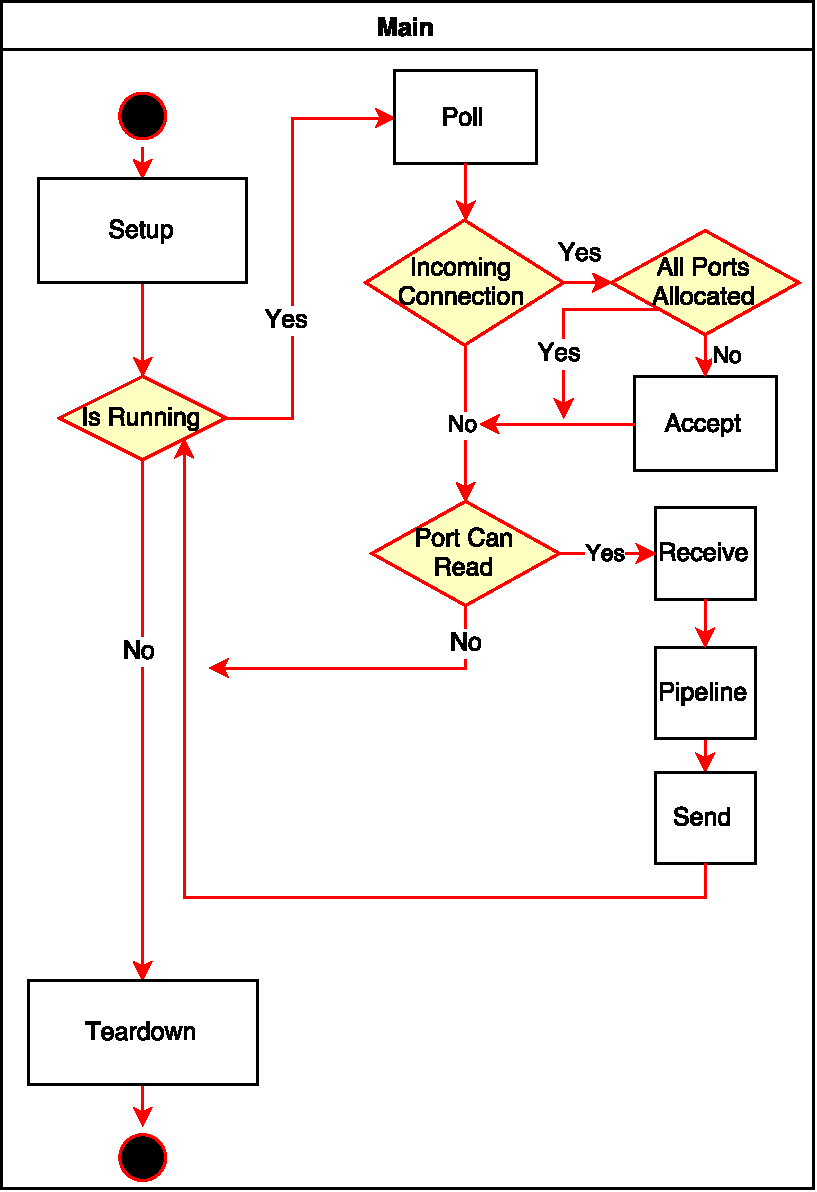
\includegraphics[scale=.8]{wire_sta_diag}
  \caption{The Freeflow STA wire state machine.}
  \label{wire_sta_diag}
\end{figure}

\subsection{Thread Per Port}
\label{expr:models-port}
In a thread per port (TPP) model, the server and FFVM ports are separated to
allow packet I/O to operate asynchronously. The main thread from the driver
handles the acceptance of new connections to the server and spawns a new thread
to execute the port work routine over them. Figure \ref{wire_tpp_diag}
illustrates the TPP wire driver process.

\begin{figure}[h!]
  \centering
  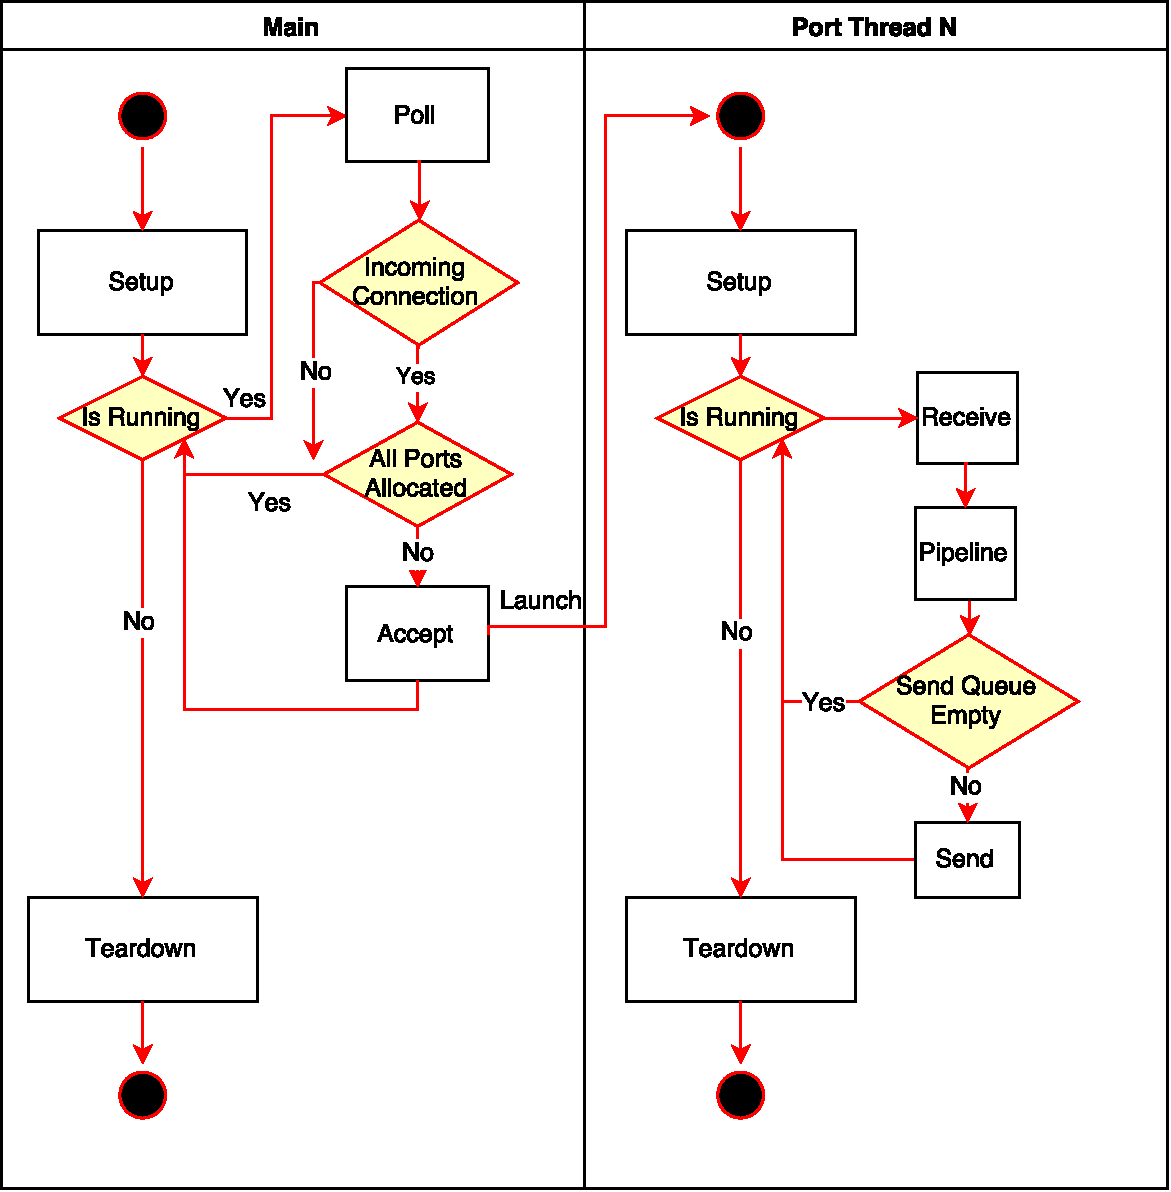
\includegraphics[scale=.75]{wire_tpp_diag}
  \caption{The Freeflow TPP wire state machine.}
  \label{wire_tpp_diag}
\end{figure}

\section{Results}
\label{expr:results}
The evaluation of the experiments conducted focuses on the measured performance
of each application with respect to throughput and bandwidth. Throughput is
defined as the number of packets per second (Pps) sent or received and
bandwidth as the amount of data in Gigabits per second (Gbps) sent or
received.

\subsection{Endpoint}
\label{expr:results:endpoint}
In the endpoint test, the average send and receive rates for throughput and
bandwidth between a baseline (Flowcap to Flowcap) and the Freeflow (Flowcap to
Endpoint) implementations are measured. This test helps measure the maximum rate
that the FFVM can provide to a hosted application. Table
\ref{endpoint_performance} lists the observed performance for both of the
testing scenarios.

\begin{table}[h!]
  \centering
  \begin{tabular}{| C{3 cm} | C{2.6cm} | C{3.1cm} | C{2.7cm} | C{3.3cm} |}
    \hline
    Implementation & Pps Received & Pps Transmitted & Gbps Received & Gbps Transmitted \\ [0.5ex]
    \hline
    Baseline & 2061814 & 2058960  & 10.167 & 10.152\\
    \hline
    Freeflow & 650864 & 707885 & 3.209 & 3.490 \\
    \hline
  \end{tabular}
  \caption{Freeflow endpoint driver and traffic generator performance metrics
  with respect to throughput and bandwidth.}
  \label{endpoint_performance}
\end{table}

The simple end-to-end connection created by the two Flowcap applications in the
baseline example shows that the sink is able to process data faster than the
source can send. Thus the rate at which packets can be received is bounded
by the rate at which they can be sent. Utilizing the Freeflow Endpoint
application introduces some overhead, as a more complex processing model is
used. These findings are shown in Table \ref{endpoint_cost}, listing the cost
in overhead between the source and sink throughput and bandwidth rates.

\begin{table}[h!]
  \centering
  \begin{tabular}{| C{3.5cm} | C{3cm} | C{3cm} |}
    \hline
    Implementation & Throughput $\Delta$ & Bandwidth $\Delta$ \\ [0.5ex]
    \hline
    Baseline & 0.139\% & 0.148\% \\
    \hline
    Freeflow & -8.055\% & -8.052\% \\
    \hline
  \end{tabular}
  \caption{Flowcap and Freeflow endpoint overhead cost with respect to
  throughput, Pps, and bandwidth, Gbps.}
  \label{endpoint_cost}
\end{table}

\subsection{Wire}
\label{expr:results:wire}
The Freeflow wire test evaluates the performance within the FFVM while hosting
an application. For the purpose of this experiment the baseline case, the STA
wire driver, is compared against the performance of the multiple versions of
the TPP wire driver. Each TPP driver version corresponds to different shared
resource strategies implemented. TPP-1 uses locked queues and copies the
context on each push/pop, while TPP-2 utilizes lock-free queues. In TPP-3,
lock-free queues hold containers of reusable buffer ids that are cached by each
thread locally. Table \ref{wire_performance} lists the observed performance
for all four of the Freeflow wire implementations tested.

\begin{table}[h]
  \centering
  \begin{tabular}{| C{2.5cm} | C{2.5cm} | C{2.5cm} | C{2.5cm} | C{2.5cm} |}
   \hline
   Architecture & Pps Received & Pps Transmitted & Gbps Received & Gbps Transmitted \\ [0.5ex]
   \hline
   STA & 504829 & 504829 & 1.861 & 1.861 \\
   \hline
   TPP-1 & 272515 & 121233 & 0.744 & 0.743 \\
   \hline
   TPP-2 & 627801 & 627801 & 3.025 & 3.025 \\
   \hline
   TPP-3 & 836129 & 950435 & 2.947 & 3.559 \\ [1ex]
   \hline\hline
   Speedup & 1.66 & 1.88 & 1.58 & 1.91 \\ [1ex]
   \hline
\end{tabular}
\caption{Freeflow wire driver performance metrics, including relative speedup.}
\label{wire_performance}
\end{table}

With each version of the TPP wire driver, the resulting performance of the FFVM
hosted application changes. The initial TPP version resulted in a major slowdown
with respect to packet throughput, but that issue was resolved by the use of
lock-free queue structures in the second version. The final version implements
more optimizations and results in the transmission rate
exceeding the reception rate in terms of throughput and bandwidth.

\section{Discussion}
\label{expr:discussion}

% Why is it slow?

The results found in the previous section show that the FFVM is a bit behind in
terms of performance. This can be attributed to numerous factors with the
experimental setups in the execution environment. In each experiment run, all
of the processes used are executed on the same device. System overhead from
the operating system juggling multiple processes does not allow for optimal
execution. This is obvious when comparing the results of the endpoint
application, as the Flowcap processes are much more light weight and less
burdensome on the OS. Adding to this is the reliance on the Linux networking
stack when using TCP (stream) sockets provided in the system API.

% Where can we move the FFVM on the spectrum to improve performance?

In order to boost performance in the FFVM, the implementation needs to be further towards the hardware end of the virtualization-materialization spectrum. Translating as much high level code down to native machine code provides the best execution environment for networking applications. For instance, flow tables can be crafted from hardware components, such as TCAMs, and manipulated by application logic. The fewer times the application-run time boundary is crossed, the more efficient the code will be executed.

% What would that mean for the ABI and portability?

However as we drift further towards a more realized implementation, we sacrifice portability for performance. This increases the amount of work that must be done by compilers to efficiently generate optimized native machine code. Additional concurrency models could also be supported by a shift towards the lower end of the spectrum, where new and exotic switch architectures sport cutting edge processors and accelerators.

% How does that affect different concurrency models?
